\documentclass{llncs}
\usepackage{amsmath,amssymb,calc,ifthen}
\usepackage{float}
%\usepackage{cancel}
\usepackage[table,usenames,dvipsnames]{xcolor} % for coloured cells in tables
\usepackage{tikz}
% Allows us to click on links and references!
\usepackage{hyperref}
\usepackage{url}
\hypersetup{
colorlinks,
citecolor=black,
filecolor=black,
linkcolor=black,
urlcolor=black
}
% Nice package for plotting graphs
% See excellent guide:
% http://www.tug.org/TUGboat/tb31-1/tb97wright-pgfplots.pdf
\usetikzlibrary{plotmarks,shapes}
\usepackage{amsmath,graphicx}
\usepackage{epstopdf}
\usepackage{caption}
\usepackage{subcaption}
\usepackage{graphicx}
% highlight - useful for TODOs and similar
\usepackage{color}
\newcommand{\hilight}[1]{\colorbox{yellow}{#1}}
\newcommand\ci{\perp\!\!\!\perp} % perpendicular sign
\newcommand*\rfrac[2]{{}^{#1}\!/_{#2}} % diagonal fraction
\newcommand\SLASH{\char`\\}
\usepackage{listings}
% margin size
\usepackage{pdfpages}
\usepackage{enumitem} % for nested enumerate numbers 1 1.1 1.1.1
% \usepackage{breqn}
% \usepackage[linesnumbered]{algorithm2e}
% \usepackage{algorithmicx,algpseudocode}
% \usepackage{wrapfig} % for allowing text wrapped around the algorithm
% \newcommand\mycommfont[1]{\footnotesize\ttfamily\textcolor{blue}{#1}}
% \SetCommentSty{mycommfont}

% \usepackage{titlesec}
% \titlespacing*{\section}
% {0pt}{5.5ex plus 1ex minus .2ex}{4.3ex plus .2ex}


\DeclareMathOperator*{\argmin}{arg\,min}
\DeclareMathOperator*{\argmax}{arg\,max}

\begin{document}

\definecolor{blue3}{HTML}{86B7FC} % med blue
\definecolor{blue1}{HTML}{B5F1FF} % light blue
\definecolor{blue2}{HTML}{E0F9FF} % very light blue

\title{Disease Knowledge Transfer for Alzheimer's Variants}
%
\titlerunning{Disease Knowledge Transfer for Alzheimer's Variants}  % abbreviated title (for running head)
%                                     also used for the TOC unless
%                                     \toctitle is used
%
\author{R\u{a}zvan V. Marinescu\inst{1} \and Pere P. Morell\inst{1} \and
Marco Lorenzi\inst{1,4} \and Neil P. Oxtoby\inst{1} \and Alexandra L. Young\inst{1} \and Arman Eshaghi\inst{1,2} \and Timothy J. Shakespeare\inst{3} \and Kier X. X. Yong\inst{3} \and Sebastian J. Crutch\inst{3} \and Daniel C. Alexander\inst{1}, for 
the  Alzheimer’s  Disease  Neuroimaging Initiative\thanks{Data used in preparation of this article were obtained from the Alzheimer's Disease Neuroimaging Initiative (ADNI) database (adni.loni.usc.edu). As such, the investigators within the ADNI contributed to the design and implementation of ADNI and/or provided data but did not participate in analysis or writing of this report. A complete listing of ADNI investigators can be found at: http://adni.loni.usc.edu/wp-content/uploads/how\_to\_apply/ADNI\_Acknowledgement\_List.pdf}}

%
\authorrunning{R\u{a}zvan V. Marinescu et al.} % abbreviated author list (for running head)
%
%%%% list of authors for the TOC (use if author list has to be modified)
% \tocauthor{Ivar Ekeland, Roger Temam, Jeffrey Dean, David Grove,
% Craig Chambers, Kim B. Bruce, and Elisa Bertino}
%
\institute{Centre for Medical Image Computing, Computer Science Department, University College London, UK
\and 
Queen Square MS Centre, UCL Institute of Neurology, London
\and 
Dementia Research Centre, UCL Institute of Neurology, University College London, UK
\and
University of C\^{o}te d'Azur, Inria Sophia Antipolis, Asclepios Research Project
% Laboratoire d'Analyse Num\'{e}rique, B\^{a}timent 425,\\
% F-91405 Orsay Cedex, France}
}

\maketitle              % typeset the title of the contribution

\begin{abstract}
% The abstract should summarize the contents of the paper
% using at least 70 and at most 150 words. It will be set in 9-point
% font size and be inset 1.0 cm from the right and left margins.
% There will be two blank lines before and after the Abstract. \dots

%5. achievement: we built a voxelwise disease progression model that uses sigmoidal traj
%6. model groups together vertices into clusters and builds a common trajectory for all vertices in the cluster
%7. Simulations show bla bla ...
%8. Tested the model on ADNI and stages correlate well with cognitive tests.
%9. Compared the patterns of typical and atypical AD with DRC data

% The model highlights, for the first time, groups of brain vertices that exhibit a similar temporal trajectory over the population. This provides a new way to parcellate the brain that is specific to the temporal trajectory of a particular disease

%%% MAX NR OF WORDS USED, DO NOT ADD MORE %%%%%%

We present Disease Knowledge Transfer (DKT), a technique for transferring biomarker correlations between Alzheimer's disease (AD) variants. DKT allows, for the first time, to infer biomarker values and their progressions in rare variants of AD for which data on such biomarkers is not available, by learning them from a different disease. For doing this, we formulate a new dementias paradigm called "Affected Overlap", which proposes that dementias are diseases that affect overlapping brain regions, and thus present certain biomarker characteristics that are shared and can thus be transferred across diseases. We then formulate the DKT model implementing this paradigm as a joint-disease generative model of biomarker progression which disentangles the biomarker correlations that are disease-specific from those correlations that are disease-agnostic. We demonstrate DKT on three datasets: (1) the TADPOLE Challenge dataset containing typical AD subjects (tAD) from the Alzheimer's Disease Neuroimaging Initiative (ADNI) dataset who had MRI, FDG, AV45, AV1451 or DTI scans, as well as two datasets from our local centre containing subjects with (2) typical AD and (3) Posterior Cortical Atrophy (PCA) that have only undergone MRI scans. We train the DKT model on all three datasets at once, and show that it is able to predict, in PCA subjects, plausible population-level biomarker for FDG, DTI, AV45 and AV1451 biomarkers, for which no data was available. We validate the predictions of DKT using a small set of DTI scans for the PCA cohort. Finally, DKT can be a useful tool to analyse and understand rare forms of dementias for which multimodal data is not available or is limited (e.g. cross-sectional). Finally, by leveraging data from multiple diseases, DKT also has the potential to provide more accurate disease staging compared to traditional disease progression models, which is useful for patient stratification in clinical trials.


\keywords{Disease Progression Model, Transfer Learning, Manifold Learning, Alzheimer's Disease, Posterior Cortical Atrophy}
\end{abstract}

%%%%%%%%% NO LONGER THAN 12 pages!! otherwise paper will be instantly rejected %%%%%%%%

\section{Introduction}



\section{Hierarchical model of disease progression}

% alzheimer's -> not homogeneous, there are many varieties -> PCA -> 
There exist several image-based biomarkers for Alzheimer's disease that can be used to track its progression: AV45 Positron Emission Tomography (PET) measuring amyloid-plaque aggregation, AV1451 PET measuring tau tangle aggregation, Flourodeoxyglucose (FDG) PET measuring brain hypometabolism, Magnetic Resonance Imaging (MRI) measuring structural integrity and Diffusion Tensor Imaging (DTI) measuring connectivity integrity. Measuring the exact evolution of these biomarkers over the disease progression can lead to better disease staging of patients, which helps stratification in clinical trials.

% add another disease example at the end
A hypothetical model of disease progression has been previously published by \ref{jack2010hypothetical}, which proposes that the first biomarkers to become abnormal are measures of amyloid beta aggregation, followed by tau abnormalities, hypometabolism, structural MRI-based measures and finally cognitive decline. While this hypothetical model proposes a modality-specific ordering of biomarkers in typical AD, it has also been observed that within the same modality, biomarker measurements also have a spatial ordering of abnormality that correlated with Braak stages: hippocampal volumes and entorhinal measures become abnormal first, followed by other structures within the temporal lobe, followed by parietal and frontal abnormalities. Moreover, this type of spatial ordering of abnormality has been observed to differ in other Alzheimer's variants. For example, in Posterior Cortical Atrophy, posterior regions such as the occipital lobe and superior parietal regions have been shown to become affected. The network vulnerability theory proposed by \cite{seeley2009neurodegenerative} suggests that damage to specific underlying connectivity networks leads to spatially distinct patterns of neurodegeneration. However, the current understanding is that within the same brain regions, 

The framework/model assumes that within a dataset of patients with a particular form of dementia, there are certain correlations between biomarkers that are \emph{disease agnostic}. For example, atrophy in the temporal lobe usually correlates with amyloid/tau-levels within the same region or with memory impairment. This is because we believe that amyloid/tau deposition cause neurodegeneration, which then causes cognitive decline in functions related to the underlying affected areas. One can then view different neurodenegenerative diseases as affecting a different set of brain regions and their underlying connectivity networks, a view supported by previous studies (Seeley, 2009, Zhou 2012). This view suggests that one can uniquely define a disease in terms of the different subset of brain regions that it affects. However, sometimes there are \emph{digo dktseasesease-agnostic} correlations that are not confined to a single region, e.g. disconnected brains regions are known to be responsible for certain cognitive functions, or biomarker measurements in different brain regions could correlate due to underlying structural or functional connectivity. One can therefore extend the idea of disease-agostic correlations between biomarkers to region-nonspecific sets of biomarkers which we will call \emph{functional units}, because the biomarkers being related through similar function.

We propose a hierarchical model of disease progression that disentangles \emph{disease-specific} biomarker correlations from \emph{disease-agnostic} correlations. For modelling disease-agnostic correlations, we assume biomarkers are grouped into \emph{functional units}, where corelations within each unit are disease-agnostic (e.g. biomarkers corresponding to the same ROI).  Each biomarker is assigned a-priori to a specific functional unit, which corresponds to a brain region, say temporal lobe (Fig 1., bottom).  For example, biomarkers assigned to the temporal unit could be: amyloid in temporal lobe, tau in temporal lobe, MRI atrophy in temporal lobe and certain memory tests. Using a disease progression model of our choice, for each region-specific functional unit we can model the correlation of biomarkers within that functional unit (Figure 1, bottom), which allows us to reconstruct a region- or unit-specific \emph{dysfunction} progression axis which can be used for staging subjects. Finally, we express the disease specific correlations (Figure 1, top) not directly with each biomarkers, but via the dysfunction scores estimated within each functional unit.  

The proposed model is parsimonious, easily interpretable by abstracting away biomarker information intothe functional units, and can be used for \emph{disease knowledge transfer}, i.e. learning correlations in one disease from another. Our approach is inspired by transfer learning methods from machine learning, but the model is generative, easing interpretability.   


\begin{figure}[h]
 \centering
 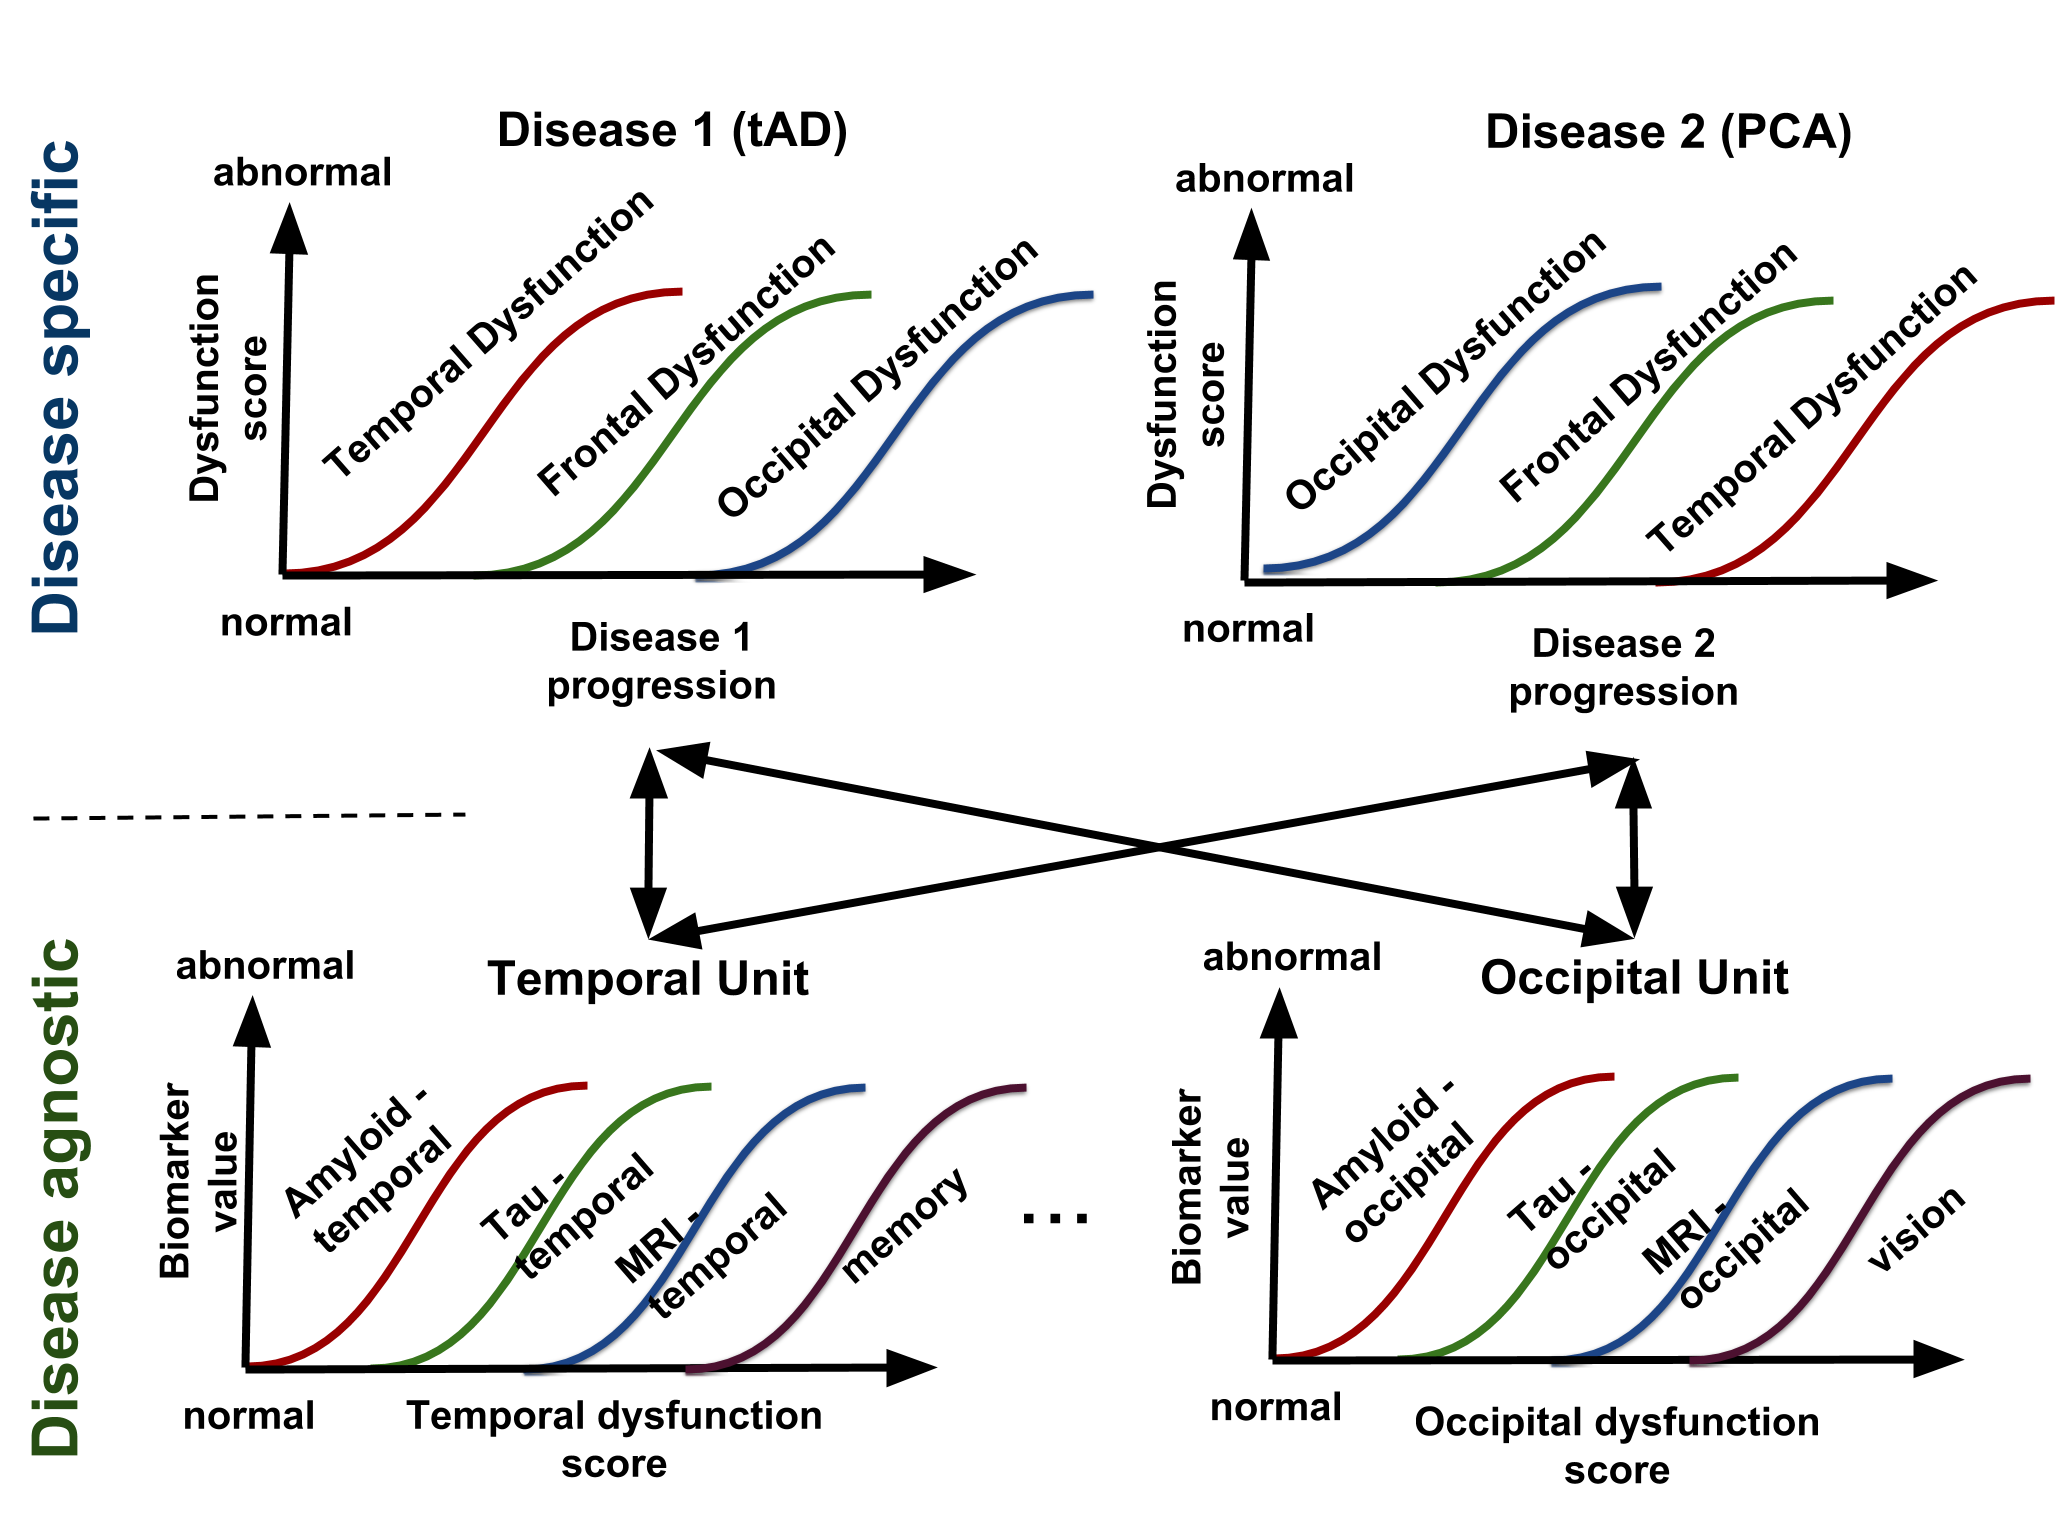
\includegraphics[height=9cm]{figures/disease_knowledge_transfer.png}
 \caption{Outline of the proposed framework for joint modelling of multiple diseases. }
\end{figure}

\subsection{Mathematical formulation}



Variable names:
\begin{itemize}
 \item $\Lambda$ = set of \emph{functional units}, i.e. \{temporal, parietal, occipital, ..\}. Biomarkers belonging to the same functional unit are asusmed to have disease-agnostic correlations.
 \item $y_{ijk}$ = measurement in subject $i$, visit $j$, biomarker $k$
%  \item $d_{ijl}$ = dysfunctionality score in subject $i$, visit $j$ in \emph{functional unit} $l$, where $l \in \Lambda$
%  \item $s_{ij}$ = disease progression score in subject $i$, visit $j$
 \item $\theta_k$ = parameters of trajectory for biomarker $k$
 \item $\lambda^l$ = parameters of trajectory for functional unit $l$, where $l \in \Lambda$
 \item $\psi$ : \{1, ..., K\} $ \rightarrow Lambda$ is a function that maps beach biomarker to its corresponding functional unit
 \item $\beta_i$: time shift parameter for subject $i$ (disease specific)
 \item $\beta_i^{l}$: time shift parameter for subject $i$ used in functional unit $l$, where $l \in \Lambda$
 \item $\Omega$: set ${(i,j,k)}$ of measurements available from every subject $i$, visit $j$ in biomarker $k$
\end{itemize}

Likelihood for one single measurement in one subject visit: 
\begin{equation}
 p(y_{ijk}|\theta_k, \lambda^{\psi(k)}, \beta_i) = \sum_{\beta_i^{\psi(k)}} p(y_{ijk}| \beta_i^{\psi(k)}, \theta_k) p(\beta_i^{\psi(k)}| \lambda^{\psi(k)}, \beta_i)
\end{equation}

where $\beta_i^{\psi(k)}$ is a latent variable denoting the stage of subject $i$ in functional unit $\psi(k)$, where biomarker $k$ was assigned.

Extending the above to multiple, subjects, visits and biomarkers, we get the final model likelihood:
\begin{equation}
 p(y_{.,.,.}|\theta_1, ..., \theta_K, \{\lambda^{\psi(l)} | l \in \Lambda \}, \beta_1, ..., \beta_N) = \prod_{(i,j,k) \in \Omega} \sum_{\beta_i^{\psi(k)}} p(y_{ijk}| \beta_i^{\psi(k)}, \theta_k) p(\beta_i^{\psi(k)}| \lambda^{\psi(k)}, \beta_i)
\end{equation}

Modelling of $p(y_{ijk}| \beta_i^{\psi(k)}, \theta_k)$ and $p(\beta_i^{\psi(k)}| \lambda^{\psi(k)}, \beta_i)$ will be done with a non-parametric model (Gaussian Process, Lorenzi et al., 2017)


\subsection*{Application 1: Disease Knowledge Transfer}

Let's assume we have MRI and PET data in tAD (from ADNI), but only MRI data for another disease, e.g. PCA. We can model the disease-agnostic region-specific relationship between MRI and PET, and also build the disease specific progression models for tAD (using MRI and PET) and PCA (using MRI only). Finally, our model allows us to propagate the knowledge of PET dynamics in tAD to PCA subjects, without using any PET scans from PCA patients. This can be done by maximising the following likelihood (assuming we already have a model for tAD):

\begin{equation}
 p(y_{.,.,.}^{PCA}|\theta_1^{tAD}, ..., \theta_K^{tAD}, \{\lambda^{\psi(l)^{PCA}} | l \in \Lambda \}, \beta_1^{PCA}, ..., \beta_N^{PCA}) = \prod_{(i,j,k) \in \Omega} \sum_{\beta_i^{\psi(k)}} p(y_{ijk}^{PCA}| \beta_i^{\psi(k)}, \theta_k^{tAD}) p(\beta_i^{\psi(k)}| \lambda^{\psi(k)^{PCA}}, \beta_i^{PCA})
\end{equation}

\subsection*{Application 2: Improved biomarker predictions and staging}

We also hope to gain improved predictions and subject staging both in all the datasets used, both the larger ones as well as the smaller ones. We can fit the models for every functional unit using all the data available in order to learn the disease-agnostic correlations between biomarkers, and then fit the disease specific progression models. Our belief is that, by using more data to inform the disease-agnostic correlations, we will get better predictions.





\section{Acknowledgements}

This work was supported by the EPSRC Centre For Doctoral Training in Medical Imaging with grant EP/L016478/1. AE received a McDonald Fellowship from the Multiple Sclerosis International Federation (MSIF, www.msif.org), and the ECTRIMS - MAGNIMS Fellowship. ALY was supported through EPSRC grant EP/J020990/01. NPO and SG received funding from the EU Horizon 2020 research and innovation programme under grant agreement No 666992. SJC was supported by an Alzheimer’s Research UK Senior Research Fellowship and ESRC/NIHR (ES/L001810/1) and EPSRC (EP/M006093/1) grants. DCA's work on this topic has funding from the EU Horizon 2020 research and innovation programme under grant agreement No 666992, as well as EPSRC grants J020990, M006093 and M020533. Data collection and sharing for this project was funded by the Alzheimer's Disease Neuroimaging Initiative (ADNI) (National Institutes of Health Grant U01 AG024904) and DOD ADNI (Department of Defense award number W81XWH-12-2-0012). The Dementia Research Centre is an ARUK coordination center.


%
% ---- Bibliography ---- 
% USE HARVARD STANDARD

\bibliographystyle{unsrtnat}
\begin{thebibliography}{5}

\bibitem{jack2010hypothetical}
Jack, C.R., Knopman, D.S., Jagust, W.J., Shaw, L.M., Aisen, P.S., Weiner, M.W., Petersen, R.C. and Trojanowski, J.Q., 2010. Hypothetical model of dynamic biomarkers of the Alzheimer's pathological cascade. The Lancet Neurology, 9(1), pp.119-128.

\bibitem{bateman2012clinical}
Bateman, R.J., Xiong, C., Benzinger, T.L., Fagan, A.M., Goate, A., Fox, N.C., Marcus, D.S., Cairns, N.J., Xie, X., Blazey, T.M. and Holtzman, D.M., 2012. Clinical and biomarker changes in dominantly inherited Alzheimer's disease. New England Journal of Medicine, 367(9), pp.795-804.

\bibitem{richberg2015multi}
Schmidt-Richberg, A., Guerrero, R., Ledig, C., Molina-Abril, H., Frangi, A.F., Rueckert, D. and Alzheimers Disease Neuroimaging Initiative, 2015, June. Multi-stage Biomarker Models for Progression Estimation in Alzheimer’s Disease. In International Conference on Information Processing in Medical Imaging (pp. 387-398). Springer International Publishing.

\bibitem{fonteijn2012event}
Fonteijn, H.M., Modat, M., Clarkson, M.J., Barnes, J., Lehmann, M., Hobbs, N.Z., Scahill, R.I., Tabrizi, S.J., Ourselin, S., Fox, N.C. and Alexander, D.C., 2012. An event-based model for disease progression and its application in familial Alzheimer's disease and Huntington's disease. NeuroImage, 60(3), pp.1880-1889.

\bibitem {jedynak2012}
Jedynak, B.M., Lang, A., Liu, B., Katz, E., Zhang, Y., Wyman, B.T., Raunig, D., Jedynak, C.P., Caffo, B., Prince, J.L. and Alzheimer's Disease Neuroimaging Initiative, 2012. A computational neurodegenerative disease progression score: method and results with the Alzheimer's Disease Neuroimaging Initiative cohort. Neuroimage, 63(3), pp.1478-1486.

\bibitem{donohue2014estimating}
Donohue, M.C., Jacqmin-Gadda, H., Le Goff, M., Thomas, R.G., Raman, R., Gamst, A.C., Beckett, L.A., Jack, C.R., Weiner, M.W., Dartigues, J.F. and Aisen, P.S., 2014. Estimating long-term multivariate progression from short-term data. Alzheimer's \& Dementia, 10(5), pp.S400-S410.

\bibitem{schiratti2015mixed}
Schiratti, J.B., Allassonniere, S., Routier, A., Colliot, O., Durrleman, S. and Alzheimers Disease Neuroimaging Initiative, 2015, June. A mixed-effects model with time reparametrization for longitudinal univariate manifold-valued data. In International Conference on Information Processing in Medical Imaging (pp. 564-575). Springer International Publishing.

\bibitem{bilgel2016multivariate}
Bilgel, M., Prince, J.L., Wong, D.F., Resnick, S.M. and Jedynak, B.M., 2016. A multivariate nonlinear mixed effects model for longitudinal image analysis: Application to amyloid imaging. NeuroImage, 134, pp.658-670.

\bibitem{seeley2009neurodegenerative}
Seeley, W.W., Crawford, R.K., Zhou, J., Miller, B.L. and Greicius, M.D., 2009. Neurodegenerative diseases target large-scale human brain networks. Neuron, 62(1), pp.42-52.

% \bibitem{bishop2006}
% Bishop, C.M., 2006. Pattern recognition. Machine Learning, 128.

\bibitem{reuter2012longitudinal}
Reuter, M., Schmansky, N.J., Rosas, H.D. and Fischl, B., 2012. Within-subject template estimation for unbiased longitudinal image analysis. Neuroimage, 61(4), pp.1402-1418.

% \bibitem{reuter2010inverse}
% Reuter, M., Rosas, H.D. and Fischl, B., 2010. Highly accurate inverse consistent registration: a robust approach. Neuroimage, 53(4), pp.1181-1196.

\bibitem{dickerson2009cortical}
Dickerson, B.C., Bakkour, A., Salat, D.H., Feczko, E., Pacheco, J., Greve, D.N., Grodstein, F., Wright, C.I., Blacker, D., Rosas, H.D. and Sperling, R.A., 2009. The cortical signature of Alzheimer's disease: regionally specific cortical thinning relates to symptom severity in very mild to mild AD dementia and is detectable in asymptomatic amyloid-positive individuals. Cerebral cortex, 19(3), pp.497-510.

% \bibitem{thompson2001cortical}
% Thompson, P.M., Mega, M.S., Woods, R.P., Zoumalan, C.I., Lindshield, C.J., Blanton, R.E., Moussai, J., Holmes, C.J., Cummings, J.L. and Toga, A.W., 2001. Cortical change in Alzheimer's disease detected with a disease-specific population-based brain atlas. Cerebral Cortex, 11(1), pp.1-16.

\bibitem{crutch2012posterior}
Crutch, S.J., Lehmann, M., Schott, J.M., Rabinovici, G.D., Rossor, M.N. and Fox, N.C., 2012. Posterior cortical atrophy. The Lancet Neurology, 11(2), pp.170-178.

\bibitem{young2015multiple}
Young, A.L., Oxtoby, N.P., Huang, J., Marinescu, R.V., Daga, P., Cash, D.M., Fox, N.C., Ourselin, S., Schott, J.M., Alexander, D.C. and Alzheimers Disease Neuroimaging Initiative, 2015, June. Multiple Orderings of Events in Disease Progression. In International Conference on Information Processing in Medical Imaging (pp. 711-722). Springer International Publishing.

\end{thebibliography}

\clearpage

\end{document}

